\documentclass[10pt,letterpaper]{article}
\usepackage[utf8]{inputenc}
\usepackage[english]{babel}
\usepackage{amsmath}
\usepackage{amsfonts}
\usepackage{amssymb}
\usepackage{graphicx}
\usepackage{verbatim}
\usepackage{listings}
\usepackage{color}
\usepackage{hyperref}

\usepackage{geometry}
\geometry{letterpaper, margin=1.0in}


\definecolor{mygreen}{rgb}{0,0.5,0}
\definecolor{mygray}{rgb}{0.9,0.9,0.9}
\definecolor{mymauve}{rgb}{0.58,0,0.82}

\lstset{ %
  backgroundcolor=\color{mygray},  % choose the background color; you must add \usepackage{color} or \usepackage{xcolor}
  basicstyle=\footnotesize,        % the size of the fonts that are used for the code
  breakatwhitespace=false,         % sets if automatic breaks should only happen at whitespace
  breaklines=true,                 % sets automatic line breaking
  captionpos=b,                    % sets the caption-position to bottom
  commentstyle=\color{mygreen},    % comment style
  deletekeywords={...},            % if you want to delete keywords from the given language
  escapeinside={\%*}{*)},          % if you want to add LaTeX within your code
  extendedchars=true,              % lets you use non-ASCII characters; for 8-bits encodings only, does not work with UTF-8
  frame=single,	                   % adds a frame around the code
  keepspaces=true,                 % keeps spaces in text, useful for keeping indentation of code (possibly needs columns=flexible)
  keywordstyle=\color{blue},       % keyword style
  language=bash,                 % the language of the code
  otherkeywords={*,...},            % if you want to add more keywords to the set
  numbers=left,                    % where to put the line-numbers; possible values are (none, left, right)
  numbersep=5pt,                   % how far the line-numbers are from the code
  numberstyle=\tiny\color{mygray}, % the style that is used for the line-numbers
  rulecolor=\color{black},         % if not set, the frame-color may be changed on line-breaks within not-black text (e.g. comments (green here))
  showspaces=false,                % show spaces everywhere adding particular underscores; it overrides 'showstringspaces'
  showstringspaces=false,          % underline spaces within strings only
  showtabs=false,                  % show tabs within strings adding particular underscores
  stepnumber=2,                    % the step between two line-numbers. If it's 1, each line will be numbered
  stringstyle=\color{mymauve},     % string literal style
  tabsize=2,	                   % sets default tabsize to 2 spaces
  title=\lstname                   % show the filename of files included with \lstinputlisting; also try caption instead of title
}







\author{Li Tai Fang / li\_tai.fang@roche.com}

\title{SomaticSeq Documentation}

\begin{document}

\maketitle



\begin{sloppypar}




\section{Introduction} \label{Introduction}

SomaticSeq is a flexible post-somatic-mutation-calling algorithm for improved accuracy. We have incorporated 10+ somatic mutation caller(s). Any combinatin of them can be used to obtain a combined call set, and then SomaticSeq uses machine learning (adaptive boosting) to distinguish true mutations from false positives from that call set. The mutation callers we have incorporated are MuTect/Indelocator/MuTect2, VarScan2, JointSNVMix, SomaticSniper, VarDict, MuSE, LoFreq, Scalpel, Strelka, and TNscope. You may incorporate some or all of those callers into your own pipeline with SomaticSeq.

The manuscript, An ensemble approach to accurately detect somatic mutations using SomaticSeq, was published in \href{http://dx.doi.org/10.1186/s13059-015-0758-2}{Genome Biology 2015, 16:197}. 
The SomaticSeq project is located at \href{https://github.com/bioinform/somaticseq}{\textit{https://github.com/bioinform/somaticseq}}. 
There have been some major improvements in SomaticSeq since that Genome Biology publication in 2015. 

SomaticSeq.Wrapper.sh is a bash script that calls a series of algorithms to combine the output of the somatic mutation caller(s). Then, depending on the input files and R scripts that are fed to SomaticSeq.Wrapper.sh, it will either 1) train the call set into a classifier, 2) predict high-confidence somatic mutations from the call set based on a pre-defined classifier, or 3) simply label the calls (i.e., PASS, LowQual, or REJECT) based on majority vote of the tools.

\subsection{Dependencies}

\begin{itemize}

\item
Python 3, plus regex, pysam, numpy, and scipy libraries. All the .py scripts are written in Python 3.

\item
R, plus the \href{https://cran.r-project.org/package=ada}{ada} package in R.

\item
BEDTools (if inclusion and/or an exclusion region files are supplied)

\item
Optional: dbSNP in VCF format (if you want to use dbSNP membership as a part of the training).

\item
At least one of MuTect/Indelocator/MuTect2, VarScan2, JointSNVMix2, SomaticSniper, VarDict, MuSE, LoFreq, Scalpel, Strelka2 and/or TNscope. Those are the tools we have incorporated in SomaticSeq. If there are other somatic tools that may be good addition to our list, please make the suggestion to us. 

\end{itemize}


\subsection{Docker images}

SomaticSeq and most somatic mutation callers we have incorporated are dockerized. 

\begin{itemize}

  \item SomaticSeq:    \href{https://hub.docker.com/r/lethalfang/somaticseq}{https://hub.docker.com/r/lethalfang/somaticseq}
  
  \item MuTect2:       \href{https://hub.docker.com/r/broadinstitute/gatk}{https://hub.docker.com/r/broadinstitute/gatk}

  \item VarScan2:      \href{https://hub.docker.com/r/djordjeklisic/sbg-varscan2}{https://hub.docker.com/r/djordjeklisic/sbg-varscan2}

  \item JointSNVMix2:  \href{https://hub.docker.com/r/lethalfang/jointsnvmix2}{https://hub.docker.com/r/lethalfang/jointsnvmix2}

  \item SomaticSniper: \href{https://hub.docker.com/r/lethalfang/somaticsniper}{https://hub.docker.com/r/lethalfang/somaticsniper}

  \item VarDict:       \href{https://hub.docker.com/r/lethalfang/vardictjava}{https://hub.docker.com/r/lethalfang/vardictjava}

  \item MuSE:          \href{https://hub.docker.com/r/marghoob/muse}{https://hub.docker.com/r/marghoob/muse}

  \item LoFreq:        \href{https://hub.docker.com/r/marghoob/lofreq}{https://hub.docker.com/r/marghoob/lofreq}

  \item Scalpel:       \href{https://hub.docker.com/r/lethalfang/scalpel}{https://hub.docker.com/r/lethalfang/scalpel}

  \item Strelka2:      \href{https://hub.docker.com/r/lethalfang/strelka}{https://hub.docker.com/r/lethalfang/strelka}

\end{itemize}


\section{How to use SomaticSeq.Wrapper.sh} \label{Wrapper_script}

The SomaticSeq.Wrapper.sh is a wrapper script that calls a series of programs and procedures \textbf{after} you have run your individual somatic mutation callers. Section \ref{dockerized_callers} will teach you how to run those mutation callers that have been dockerized. It also includes ways to create semi-simulated training data that can be used to create SomaticSeq classifiers. In the next section, we will describe the workflow in this wrapper script in detail, so you may not be dependent on this wrapper script. You can either modify this wrapper script or create your own workflow using whatever workflow language you want. 


\subsection{SomaticSeq Training Mode} \label{somaticseq_train}

To create SomaticSeq classifiers, you need VCF files containing true positive SNVs and INDELs. There is also an option to include a list of regions to include and/or exclude from this exercise. The exclusion or inclusion regions can be VCF or BED files. An inclusion region may be subset of the call sets where you have validated their true/false mutation status, so that only those regions will be used for training. An exclusion region can be regions where the ``truth'' is ambigious. All the variants in the truth VCF files are assumed to be true positives. Every mutation call not in the truth VCF files is assumed to be false positives (as long as the genomic coordiante is in inclusion region and not in exclusion region if those regions are provided). 

All the output VCF files from individual callers are optional. Those VCF files can be bgzipped if they have .vcf.gz extensions. It is imperative that you will use the same parameter for prediction as you do for training. 

\begin{lstlisting}
# An example: for training, truth file and the correct R script are required.

SomaticSeq.Wrapper.sh \
--mutect2           MuTect2/variants.vcf \
--varscan-snv       VarScan2/variants.snp.vcf \
--varscan-indel     VarScan2/variants.indel.vcf \
--jsm               JointSNVMix2/variants.snp.vcf \
--sniper            SomaticSniper/variants.snp.vcf \
--vardict           VarDict/variants.vcf \
--muse              MuSE/variants.snp.vcf \
--lofreq-snv        LoFreq/variants.snp.vcf \
--lofreq-indel      LoFreq/variants.indel.vcf \
--scalpel           Scalpel/variants.indel.vcf \
--strelka-snv       Strelka/variants.snv.vcf \
--strelka-indel     Strelka/variants.indel.vcf \
--tnscope           TNscope.vcf.gz \
--normal-bam        matched_normal.bam \
--tumor-bam         tumor.bam \
--ada-r-script      $somaticseq/r_scripts/ada_model_builder_ntChange.R \
--genome-reference  GRCh38.fa \
--cosmic            cosmic.GRCh38.vcf \
--dbsnp             dbSNP.GRCh38.vcf \
--exclusion-region  blackList.bed \
--inclusion-region  highConfidenceRegions.bed
--truth-snv         truePositives.snv.vcf \
--truth-indel       truePositives.indel.vcf \
--output-dir        $OUTPUT_DIR
\end{lstlisting}

SomaticSeq.Wrapper.sh supports any combination of the somatic mutation callers we have incorporated into the workflow. SomaticSeq will run based on the output VCFs you have provided. It will train for SNV and/or INDEL if you provide the truePositives.snv.vcf and/or truePositives.indel.vcf file(s) as well as the proper R script (ada\_model\_builder\_ntChange.R). Otherwise, it will fall back to the simple caller consensus mode.




\subsection{SomaticSeq Prediction Mode} \label{somaticseq_prediction}

Make sure the classifiers (.RData files) and the proper R script (ada\_model\_predictor.R) are supplied, Without either of them, it will fall back to the simple caller consensus mode.


\begin{lstlisting}
# The *.RData files are trained classifier from the training mode.
SomaticSeq.Wrapper.sh \
--mutect2           MuTect2/variants.vcf \
--varscan-snv       VarScan2/variants.snp.vcf \
--varscan-indel     VarScan2/variants.indel.vcf \
--jsm               JointSNVMix2/variants.snp.vcf \
--sniper            SomaticSniper/variants.snp.vcf \
--vardict           VarDict/variants.vcf \
--muse              MuSE/variants.snp.vcf \
--lofreq-snv        LoFreq/variants.snp.vcf \
--lofreq-indel      LoFreq/variants.indel.vcf \
--scalpel           Scalpel/variants.indel.vcf \
--strelka-snv       Strelka/variants.snv.vcf \
--strelka-indel     Strelka/variants.indel.vcf \
--tnscope           TNscope.vcf.gz \
--normal-bam        matched_normal.bam \
--tumor-bam         tumor.bam \
--ada-r-script      ada_model_predictor.R \
--genome-reference  human_b37.fasta \
--genome-reference  GRCh38.fa \
--cosmic            cosmic.GRCh38.vcf \
--dbsnp             dbSNP.GRCh38.vcf \
--exclusion-region  blackList.bed \
--inclusion-region  highConfidenceRegions.bed
--classifier-snv    sSNV.Classifier.RData \
--classifier-indel  sINDEL.Classifier.RData \
--pass-threshold    0.5 \
--lowqual-threshold 0.1 \
--output-dir        $OUTPUT_DIR

\end{lstlisting}



\subsection{Consensus Mode} \label{somaticseq_default_mode}

Same as the commands previously, but not including the R script or the ground truth files. Without those information, SomaticSeq will forgo machine learning, and fall back into a simple majority vote.



\section{The step-by-step SomaticSeq Workflow} \label{step_by_step_procedures}

We'll describe the workflow here, so you may modify the workflow and/or create your own workflow (better optimized for your own usage), instead of using SomaticSeq.Wrapper.sh we have included in the repo.


\subsection{Combine the call sets}
We use utilities/getUniqueVcfPositions.py and vcfsorter.pl to combine the VCF files from different callers. For each caller output, intermediate VCF file(s) were modified separate the SNVs and INDELs calls, and also remove some REJECT calls to reduce file sizes.

\begin{enumerate}

% MuTect and Indelocator
\item 
Modify (original) MuTect and/or Indelocator output VCF files. 
Since MuTect's output VCF do not always put the tumor and normal samples in the same columns, the script will determine that information based on either the BAM files (the header has sample name information), or based on the sample information that you tell it, and then determine which column belongs to the normal, and which column belongs to the tumor. 
	
\begin{lstlisting}
# Modify MuTect and Indelocator's output VCF based on BAM files
modify_MuTect.py -infile input.vcf -outfile output.vcf -nbam normal.bam -tbam tumor.bam
	
# Based on the sample name you supply:
modify_MuTect.py -infile input.vcf -outfile output.vcf -nsm NormalSampleName -tsm TumorSampleName
\end{lstlisting}


% MuTect 2 (from GATK 4)
\item
For MuTect2, this script will split multi-allelic records into one variant per line in the VCF file. This is to make thing easier for the SSeq\_merged.vcf2tsv.py script later. 

\begin{lstlisting}
# Based on the sample name you supply:
modify_MuTect2.py -infile MuTect2.Filtered.vcf -snv mutect.snp.vcf -indel mutect.indel.vcf
\end{lstlisting}


% VarScan2
\item
Modify VarScan's output VCF files to be rigorously concordant to VCF format standard, and to attach the tag 'VarScan2' to somatic calls. 
\begin{lstlisting}
# Do it for both the SNV and indel
modify_VJSD.py -method VarScan2 -infile input.vcf -outfile output.vcf
\end{lstlisting}


% JointSNVMix2
\item
JointSNVMix2 does not output VCF files. In our own \href{https://github.com/bioinform/somaticseq/blob/master/utilities/dockered_pipelines/mutation_callers/submit_JointSNVMix2.sh}{workflow}, we convert its output into a basic VCF file with an 2 awk one-liners, which you may see at utilities/dockered\_pipelines/mutation\_callers/submit\_JointSNVMix2.sh.

\begin{lstlisting}
# To avoid text files on the order of terabytes, this awk one-liner keeps entries where the reference is not "N", and the somatic probabilities are at least 0.95.
awk -F "\t" 'NR!=1 && $4!="N" && $10+$11>=0.95'
	
# This awk one-liner converts the text file into a basic VCF file
awk -F "\t" '{print $1 "\t" $2 "\t.\t" $3 "\t" $4 "\t.\t.\tAAAB=" $10 ";AABB=" $11 "\tRD:AD\t" $5 ":" $6 "\t" $7 ":" $8}'

## The actual commands we've used in our workflow:
echo -e '##fileformat=VCFv4.1' > unsorted.vcf
echo -e '##INFO=<ID=AAAB,Number=1,Type=Float,Description="Probability of Joint Genotype AA in Normal and AB in Tumor">' >> unsorted.vcf
echo -e '##INFO=<ID=AABB,Number=1,Type=Float,Description="Probability of Joint Genotype AA in Normal and BB in Tumor">' >> unsorted.vcf
echo -e '##FORMAT=<ID=RD,Number=1,Type=Integer,Description="Depth of reference-supporting bases (reads1)">' >> unsorted.vcf
echo -e '##FORMAT=<ID=AD,Number=1,Type=Integer,Description="Depth of variant-supporting bases (reads2)">' >> unsorted.vcf
echo -e '#CHROM\tPOS\tID\tREF\tALT\tQUAL\tFILTER\tINFO\tFORMAT\tNORMAL\tTUMOR' >> unsorted.vcf

python $PATH/TO/jsm.py classify joint_snv_mix_two genome.GRCh37.fa normal.bam tumor.bam trained.parameter.cfg /dev/stdout |\
awk -F "\t" 'NR!=1 && $4!="N" && $10+$11>=0.95' |\
awk -F "\t" '{print $1 "\t" $2 "\t.\t" $3 "\t" $4 "\t.\t.\tAAAB=" $10 ";AABB=" $11 "\tRD:AD\t" $5 ":" $6 "\t" $7 ":" $8}' >> unsorted.vcf
\end{lstlisting}
	
After that, you'll also want to sort the VCF file.
	
\begin{lstlisting}
modify_VJSD.py -method JointSNVMix2 -infile input.vcf -outfile output.vcf
\end{lstlisting}

% SomaticSniper:
\item	
Modify SomaticSniper's output:

\begin{lstlisting}
modify_VJSD.py -method SomaticSniper -infile input.vcf -outfile output.vcf
\end{lstlisting}


% VarDict
\item	
VarDict has both SNV and indel, plus some other variants in the same VCF file. Our script will create two files, one for SNV and one for indel, while everything else is ignored for now. By default, LikelySomatic/StrongSomatic and PASS calls will be labeled VarDict. However, in our SomaticSeq paper, based on our experience in DREAM Challenge, we implemented two custom filters to relax the VarDict tagging criteria. 


\begin{lstlisting}
# Default VarDict tagging criteria, only PASS (and Likely or Strong Somatic):
modify_VJSD.py -method VarDict -infile intput.vcf -outfile output.vcf
	
# When running VarDict, if var2vcf_paired.pl is used to generate the VCF file, you may relax the tagging criteria with -filter paired
modify_VJSD.py -method VarDict -infile intput.vcf -outfile output.vcf -filter paired
	
# When running VarDict, if var2vcf_somatic.pl is used to generate the VCF file, you may relax the tagging criteria with -filter somatic
modify_VJSD.py -method VarDict -infile intput.vcf -outfile output.vcf -filter somatic
\end{lstlisting}
	

In the SomaticSeq paper, -filter somatic was used because var2vcf\_somatic.pl was used to generate VarDict's VCF files. In the SomaticSeq.Wrapper.sh script, however, -filter paired is used because VarDict authors have since recommended var2vcf\_paired.pl script to create the VCF files. While there are some differences (different stringencies in some filters) in what VarDict labels as PASS between the somatic.pl and paired.pl scripts, the difference is miniscule after applying our custom filter (which relaxes the filter, resulting in a difference about 5 calls out of 15,000). 

The output files will be snp.output.vcf and indel.output.vcf. 


% MuSE
\item
MuSE was not a part of our analysis in the SomaticSeq paper. We have implemented it later. 
	
\begin{lstlisting}
modify_VJSD.py -method MuSE -infile input.vcf -outfile output.vcf
\end{lstlisting}


% LoFreq
\item
LoFreq and Scalpel do not require modification. LoFreq has no sample columns anyway. 


% Strelka
\item
Add ``GT'' field to sample columns to make it compatible with GATK CombineVariants.

\begin{lstlisting}
modify_Strelka.py -infile somatic.snvs.vcf.gz -outfile stralka.snv.vcf
\end{lstlisting}


% GATK CombineVariants
\item
Finally, with the VCF files modified, you need combine them: one for SNV and one for indel separately.
	
\begin{lstlisting}
# Combine the VCF files for SNV. Any or all of the VCF files may be present.
utilities/getUniqueVcfPositions.py -vcfs mutect.vcf varscan.snp.vcf jointsnvmix.vcf snp.vardict.vcf muse.vcf -out CombineVariants.snp.vcf
\end{lstlisting}


\end{enumerate}





\subsection{Apply inclusion and exclusion regions}

This step may be needed for model training. The workflow in SomaticSeq.Wrapper.sh allows for inclusion and exclusion region. An inclusion region means we will only use calls inside these regions. An exclusion region means we do not care about calls inside this region. DREAM Challenge had exclusion regions, e.g., blacklisted regions, etc. 
	
\begin{lstlisting}
# In the DREAM_Stage_3 directory, we have included an exclusion region BED file as an example
# This command uses BEDtools to rid of all calls in the exclusion region
intersectBed -header -a BINA_somatic.snp.vcf   -b ignore.bed -v > somatic.snp.processed.vcf
intersectBed -header -a BINA_somatic.indel.vcf -b ignore.bed -v > somatic.indel.processed.vcf

# Alternatively (or both), this command uses BEDtools to keep only calls in the inclusion region
intersectBed -header -a BINA_somatic.snp.vcf   -b inclusion.bed > somatic.snp.processed.vcf
intersectBed -header -a BINA_somatic.indel.vcf -b inclusion.bed > somatic.indel.processed.vcf

\end{lstlisting}



\subsection{Convert the VCF file into TSV file}
This script works for all VCF files. It extracts information from BAM files, as well as some individual callers' output VCF files. If the ground truth VCF file is included, a called variant will be annotated as a true positive, and everything will be annotated as a false positive.

	
\begin{lstlisting}
# SNV
SSeq_merged.vcf2tsv.py -ref genome.GRCh37.fa -myvcf somatic.snp.processed.vcf -truth Ground.truth.snp.vcf -mutect MuTect/variants.snp.vcf.gz -varscan VarScan2/variants.snp.vcf -jsm JSM2/variants.vcf -sniper SomaticSniper/variants.vcf -vardict VarDict/snp.variants.vcf -muse MuSE/variants.vcf -lofreq LoFreq/variants.snp.vcf -strelka Strelka/variants.snp.vcf -dedup -tbam tumor.bam -nbam normal.bam -outfile Ensemble.sSNV.tsv
\end{lstlisting}


That was for SNV, and indel is almost the same thing. After version 2.1, we have replaced all information from SAMtools and HaplotypeCaller with information directly from the BAM files. The accuracy differences are negligible with significant improvement in usability and resource requirement.

\begin{lstlisting}
# INDEL:
SSeq_merged.vcf2tsv.py -ref genome.GRCh37.fa -myvcf somatic.indel.processed.vcf -truth Ground.truth.indel.vcf -varscan VarScan2/variants.snp.vcf -vardict VarDict/indel.variants.vcf -lofreq LoFreq/variants.indel.vcf -scalpel Scalpel/variants.indel.vcf -strelka Strelka/variants.indel.vcf -tbam tumor.bam -nbam normal.bam -dedup -outfile Ensemble.sINDEL.tsv
\end{lstlisting}


At the end of this, Ensemble.sSNV.tsv and Ensemble.sINDEL.tsv are created. 

All the options for SSeq\_merged.vcf2tsv.py are listed here. They can also be displayed by running SSeq\_merged.vcf2tsv.py \texttt{--}help.

\begin{lstlisting}

  -myvcf       Input VCF file of the merged calls [REQUIRED]
  -ref         Genome reference fa/fasta file [REQUIRED]
  -nbam        BAM file of the matched normal sample [REQUIRED]
  -tbam        BAM file of the tumor sample [REQUIRED]
  -ref         Genome reference fa/fastq file [REQUIRED]
  -truth       Ground truth VCF file. Every other position is a False Positive.
  -dbsnp       dbSNP VCF file
  -cosmic      COSMIC VCF file
  -mutect      VCF file from either MuTect2, MuTect, or Indelocator
  -sniper      VCF file from SomaticSniper
  -varscan     VCF file from VarScan2
  -jsm         VCF file from Bina's workflow that contains JointSNVMix2
  -vardict     VCF file that contains only SNV or only INDEL from VarDict
  -muse        VCF file from MuSE
  -lofreq      VCF file from LoFreq
  -scalpel     VCF file from Scalpel
  -strelka     VCF file from Strelka
  -dedup       A flag to consider only primary reads
  -minMQ       Minimum mapping quality for reads to be considered (Default = 1)
  -minBQ       Minimum base quality for reads to be considered (Default = 5)
  -mincaller   Minimum number of caller classification for a call to be considered (Use 0.5 to consider some LowQual calls. Default = 0).
  -scale       The options are phred, fraction, or None, to convert numbers to Phred scale or fractional scale. (default = None, i.e., no conversion)
  -outfile     Output TSV file name
                        
\end{lstlisting}


Note: Do not worry if Python throws a warning like this. 

\begin{lstlisting}
RuntimeWarning: invalid value encountered in double_scalars
  z = (s - expected) / np.sqrt(n1*n2*(n1+n2+1)/12.0)
\end{lstlisting}

This is to tell you that scipy was attempting some statistical test with empty data. That's usually due to the fact that normal BAM file has no variant reads at that given position. That is why lots of values are NaN for the normal. 




\subsection{Model Training or Mutation Prediction}

You can use Ensemble.sSNV.tsv and Ensemble.sINDEL.tsv files either for model training (provided that their mutation status is annotated with 0 or 1) or mutation prediction. This is done with stochastic boosting algorithm we have implemented in R. 
	
Model training:
\begin{lstlisting}
# Training:
r_scripts/ada_model_builder_ntChange.R Ensemble.sSNV.tsv   Consistent_Mates Inconsistent_Mates
r_scripts/ada_model_builder_ntChange.R Ensemble.sINDEL.tsv Strelka_QSS Strelka_TQSS Consistent_Mates Inconsistent_Mates
\end{lstlisting}
	
Ensemble.sSNV.tsv.Classifier.RData and Ensemble.sINDEL.tsv.Classifier.RData will be created from model training. The arguments after Ensemble.sSNV.tsv and Ensemble.sINDEL.tsv tells the builder script to ignore those features in training. These features do not improve accuracy in our data sets (mostly WGS data, but they may help other data sets)
	

Mutation prediction:
	
\begin{lstlisting}
# Mutation prediction:
r_script/ada_model_predictor.R Ensemble.sSNV.tsv.Classifier.RData   Ensemble.sSNV.tsv   Trained.sSNV.tsv
r_script/ada_model_predictor.R Ensemble.sINDEL.tsv.Classifier.RData Ensemble.sINDEL.tsv Trained.sINDEL.tsv
\end{lstlisting}

	
After mutation prediction, if you feel like it, you may convert Trained.sSNV.tsv and Trained.sINDEL.tsv into VCF files. Use -tools to list ONLY the individual tools used to have appropriately annotated VCF files. Accepted tools are MuTect2/MuTect/Indelocator, VarScan2, JointSNVMix2, SomaticSniper, VarDict, MuSE, LoFreq, Scalpel, Strelka, and/or TNscope. To list a tool without having run it, the VCF will be annotated as if the tool was run but did not identify that position as a somatic variant, which is probably undesireable. 


\begin{lstlisting}
# Probability above 0.7 labeled PASS (-pass 0.7), and between 0.1 and 0.7 labeled LowQual (-low 0.1):
# Use -all to include REJECT calls in the VCF file
# Use -phred to convert probability values (between 0 to 1) into Phred scale in the QUAL column in the VCF file

SSeq_tsv2vcf.py -tsv Trained.sSNV.tsv   -vcf Trained.sSNV.vcf   -pass 0.7 -low 0.1 -tools MuTect2 VarScan2 JointSNVMix2 SomaticSniper VarDict MuSE LoFreq Strelka -all -phred

SSeq_tsv2vcf.py -tsv Trained.sINDEL.tsv -vcf Trained.sINDEL.vcf -pass 0.7 -low 0.1 -tools MuTect2 VarScan2 VarDict LoFreq Scalpel Strelka -all -phred
\end{lstlisting}



\section{To run the dockerized somatic mutation callers} \label{dockerized_callers}

For your convenience, we have created a couple of scripts that can generate run script for the dockerized somatic mutation callers. 

\subsection{Location}

  \begin{itemize}
    \item somaticseq/utilities/dockered\_pipelines/
  \end{itemize}

\subsection{Requirements}

  \begin{itemize}
    \item Have internet connection, and able to pull and run docker images from docker.io
    \item Have cluster management system such as Sun Grid Engine, so that the "qsub" command is valid
  \end{itemize}


\subsection{Example commands}


\subsubsection{Single-threaded Jobs}

This is best suited for whole exome sequencing or less. 

\begin{lstlisting}
# Example command to submit the run scripts for each of the following somatic mutation callers
$PATH/TO/somaticseq/utilities/dockered_pipelines/submit_callers_singleThread.sh \
--normal-bam      /ABSOLUTE/PATH/TO/normal_sample.bam \
--tumor-bam       /ABSOLUTE/PATH/TO/tumor_sample.bam \
--human-reference /ABSOLUTE/PATH/TO/GRCh38.fa \
--output-dir      /ABSOLUTE/PATH/TO/RESULTS \
--dbsnp           /ABSOLUTE/PATH/TO/dbSNP.GRCh38.vcf \
--somaticseq-dir  /ABSOLUTE/PATH/TO/SomaticSeq \
--action          echo \
--mutect2 --somaticsniper --vardict --muse --lofreq --scalpel --strelka --somaticseq
\end{lstlisting}
The command shown above will create scripts for MuTect2, SomaticSniper, VarDict, MuSE, LoFreq, Scalpel, and Strelka. Then, it will create the SomaticSeq script that merges those 7 callers. This command defaults to majority-vote consensus.

Since it's --aciton echo, it will echo the mutation caller scripts locations, but these scripts will not be run. If you do --action qsub instead, then those mutation caller scripts will be qsub'ed. You'll still need to mantually run/submit the SomaticSeq script after all the caller jobs are done.



\subsubsection{Multi-threaded Jobs}

This is best suited for whole genome sequencing. 
This is same as above, except it will create 36 equal-size regions in 36 bed files, and parallelize the jobs into 36 regions.

\begin{lstlisting}
# Submitting mutation caller jobs by splitting each job into 36 even regions.
$PATH/TO/somaticseq/utilities/dockered_pipelines/submit_callers_multiThreads.sh \
--normal-bam      /ABSOLUTE/PATH/TO/normal_sample.bam \
--tumor-bam       /ABSOLUTE/PATH/TO/tumor_sample.bam \
--human-reference /ABSOLUTE/PATH/TO/GRCh38.fa \
--output-dir      /ABSOLUTE/PATH/TO/RESULTS \
--dbsnp           /ABSOLUTE/PATH/TO/dbSNP.GRCh38.vcf \
--threads         36 \
--action          echo \
--mutect2 --somaticsniper --vardict --muse --lofreq --scalpel --strelka --somaticseq
\end{lstlisting}



\subsubsection{SomaticSeq Training}

Two classifiers will be created (*.RData files), one for SNV and one for INDEL.

\begin{lstlisting}
# Submitting mutation caller jobs by splitting each job into 36 even regions.
$PATH/TO/somaticseq/utilities/dockered_pipelines/submit_callers_singleThread.sh \
--normal-bam      /ABSOLUTE/PATH/TO/normal_sample.bam \
--tumor-bam       /ABSOLUTE/PATH/TO/tumor_sample.bam \
--truth-snv       /ABSOLUTE/PATH/TO/snvTruth.vcf \
--truth-indel     /ABSOLUTE/PATH/TO/indelTruth.vcf \
--human-reference /ABSOLUTE/PATH/TO/GRCh38.fa \
--output-dir      /ABSOLUTE/PATH/TO/RESULTS \
--dbsnp           /ABSOLUTE/PATH/TO/dbSNP.GRCh38.vcf \
--somaticseq-dir  /ABSOLUTE/PATH/TO/SomaticSeq \
--action          echo \
--mutect2 --somaticsniper --vardict --muse --lofreq --scalpel --strelka --somaticseq --somaticseq-train
\end{lstlisting}

Notice the command includes --truth-snv and --truth-indel, and invokes somaticseq-train.

For multi-threaded job, you should not invoke somaticseq-train. Instead, you should combine all the Ensemble.sSNV.tsv and Ensemble.sINDEL.tsv files (separately), and then train on the combined files.




\subsubsection{SomaticSeq Prediction}

\begin{lstlisting}
# Submitting mutation caller jobs by splitting each job into 36 even regions.
$PATH/TO/somaticseq/utilities/dockered_pipelines/submit_callers_singleThread.sh \
--normal-bam       /ABSOLUTE/PATH/TO/normal_sample.bam \
--tumor-bam        /ABSOLUTE/PATH/TO/tumor_sample.bam \
--classifier-snv   /ABSOLUTE/PATH/TO/Ensemble.sSNV.tsv.ntChange.Classifier.RData \
--classifier-indel /ABSOLUTE/PATH/TO/Ensemble.sINDEL.tsv.ntChange.Classifier.RData \
--human-reference  /ABSOLUTE/PATH/TO/GRCh38.fa \
--output-dir       /ABSOLUTE/PATH/TO/RESULTS \
--dbsnp            /ABSOLUTE/PATH/TO/dbSNP.GRCh38.vcf \
--somaticseq-dir   /ABSOLUTE/PATH/TO/SomaticSeq \
--action           echo \
--mutect2 --somaticsniper --vardict --muse --lofreq --scalpel --strelka --somaticseq
\end{lstlisting}

Notice the command includes --classifier-snv and --classifier-indel.







\subsubsection{Parameters}

\begin{lstlisting}
--normal-bam                  /ABSOLUTE/PATH/TO/normal_sample.bam (Required)
--tumor-bam                   /ABSOLUTE/PATH/TO/tumor_sample.bam  (Required)
--human-reference             /ABSOLUTE/PATH/TO/human_reference.fa (Required)
--dbsnp                       /ABSOLUTE/PATH/TO/dbsnp.vcf (Required for MuSE and LoFreq)
--cosmic                      /ABSOLUTE/PATH/TO/cosmic.vcf (Optional)
--selector                    /ABSOLUTE/PATH/TO/Capture_region.bed (Optional. Will assume whole genome from the .fai file without it.)
--exclude                     /ABSOLUTE/PATH/TO/Blacklist_region.bed (Optional)
--min-af                      (Optional. The minimum VAF cutoff for VarDict and VarScan2. Defaults are 0.10 for VarScan2 and 0.05 for VarDict).
--action                      qsub (Optional: the command preceding the .cmd scripts. Default is echo)
--threads                     36 (Optional for multiThreads and invalid for singleThread: evenly split the genome into 36 BED files. Default = 12).
--mutect2                     (Optional flag to invoke MuTect2)
--varscan2                    (Optional flag to invoke VarScan2)
--jointsnvmix2                (Optional flag to invoke JointSNVMix2)
--somaticsniper               (Optional flag to invoke SomaticSniper)
--vardict                     (Optional flag to invoke VarDict)
--muse                        (Optional flag to invoke MuSE)
--lofreq                      (Optional flag to invoke LoFreq)
--scalpel                     (Optional flag to invoke Scalpel)
--strelka                     (Optional flag to invoke Strelka)
--somaticseq                  (Optional flag to invoke SomaticSeq. This script always be echo'ed, as it should not be submitted until all the callers above complete).
--output-dir                  /ABSOLUTE/PATH/TO/OUTPUT_DIRECTORY (Required)
--somaticseq-dir              SomaticSeq_Output_Directory (Optional. The directory name of the SomaticSeq output. Default = SomaticSeq).
--somaticseq-train            (Optional flag to invoke SomaticSeq to produce classifiers if ground truth VCF files are provided. Only recommended in singleThread mode, because otherwise it's better to combine the output TSV files first, and then train classifiers.)
--somaticseq-action           (Optional. What to do with the somaticseq.cmd. Default is echo. Only do "qsub" if you have already completed all the mutation callers, but want to run SomaticSeq at a different setting.)
--classifier-snv              Trained_sSNV_Classifier.RData (Optional if there is a classifer you want to use)
--classifier-indel            Trained_sINDEL_Classifier.RData (Optional if there is a classifer you want to use)
--truth-snv                   sSNV_ground_truth.vcf (Optional if there is a ground truth, and everything else will be labeled false positive)
--truth-indel                 sINDEL_ground_truth.vcf (Optional if there is a ground truth, and everything else will be labeled false positive)
--exome                       (Optional flag for Strelka)
--scalpel-two-pass            (Optional parameter for Scalpel. Default = false.)
--mutect2-arguments           (Extra parameters to pass onto Mutect2, e.g., --mutect2-arguments '--initial_tumor_lod 3.0 --log_somatic_prior -5.0 --min_base_quality_score 20')
--mutect2-filter-arguments    (Extra parameters to pass onto FilterMutectCalls)
--varscan-arguments           (Extra parameters to pass onto VarScan2)
--varscan-pileup-arguments    (Extra parameters to pass onto samtools mpileup that creates pileup files for VarScan)
--jsm-train-arguments         (Extra parameters to pass onto JointSNVMix2's train command)
--jsm-classify-arguments      (Extra parameters to pass onto JointSNVMix2's classify command)
--somaticsniper-arguments     (Extra parameters to pass onto SomaticSniper)
--vardict-arguments           (Extra parameters to pass onto VarDict)
--muse-arguments              (Extra parameters to pass onto MuSE)
--lofreq-arguments            (Extra parameters to pass onto LoFreq)
--scalpel-discovery-arguments (Extra parameters to pass onto Scalpel's discovery command)
--scalpel-export-arguments    (Extra parameters to pass onto Scalpel's export command)
--strelka-config-arguments    (Extra parameters to pass onto Strelka's config command)
--strelka-run-arguments       (Extra parameters to pass onto Strekla's run command)
--somaticseq-arguments        (Extra parameters to pass onto SomaticSeq.Wrapper.sh)
\end{lstlisting}



\subsubsection{What does the single-threaded command do}

\begin{itemize}
  \item
  For each flag such as \texttt{--}mutect2, \texttt{--}jointsnvmix2, ...., \texttt{--}strelka, a run script ending with .cmd will be created in /ABSOLUTE/PATH/TO/RESULTS/logs. By default, these .cmd scripts will only be created, and their file path will be printed on screen. However, if you do ``\texttt{--}action qsub'', then these scripts will be submitted via the qsub command. The default action is ``echo.''

    \begin{itemize}
    \item Each of these .cmd script correspond to a mutation caller you specified. They all use docker images.
    \item We may improve their functionalities in the future to allow more tunable parameters. For the initial releases, POC and reproducibility take precedence.
    \end{itemize}
  
  \item
  If you do ``\texttt{--}somaticseq,'' the somaticseq script will be created in /ABSOLUTE/PATH/TO/RESULTS/SomaticSeq/logs. However, it will not be submitted until you manually do so after each of these mutation callers is finished running. 
      
    \begin{itemize}
    \item   
     In the future, we may create more sophisticated solution that will automatically solves these dependencies. For the initial release, we'll focus on stability and reproducibility. 
    \end{itemize}
  
  \item
  Due to the way those run scripts are written, the Sun Grid Engine's standard error log will record the time the task completes (i.e., Done at 2017/10/30 29:03:02), and it will only do so when the task is completed with an exit code of 0. It can be a quick way to check if a task is done, by looking at the final line of the standard error log file.

\end{itemize}



\subsubsection{What does the multi-threaded command do}
It's very similar to the single-threaded WES solution, except the job will be split evenly based on genomic lengths.

\begin{itemize}
  \item
  If you specified ``\texttt{--}threads 36,'' then 36 BED files will be created. Each BED file represents 1/36 of the total base pairs in the human genome (obtained from the .fa.fai file, but only including 1, 2, 3, ..., MT, or chr1, chr2, ..., chrM contigs). They are named 1.bed, 2.bed, ..., 36.bed, and will be created into /ABSOLUTE/PATH/TO/RESULTS/1, /ABSOLUTE/PATH/TO/RESULTS/2, ..., /ABSOLUTE/PATH/TO/RESULTS/36. You may, of course, specify any number. The default is 12.

  \item
  For each mutation callers you specify (with the exception of SomaticSniper), a script will be created into /ABSOLUTE/PATH/TO/RESULTS/1/logs, /ABSOLUTE/PATH/TO/RESULTS/2/logs, etc., with partial BAM input. Again, they will be automatically submitted if you do ``\texttt{--}action qsub.''
  
  \item
  Because SomaticSniper does not support partial BAM input (one would have to manually split the BAMs in order to parallelize SomaticSniper this way), the above mentioned procedure is not applied to SomaticSniper. Instead, a single-threaded script will be created (and potentially qsub'ed) into /ABSOLUTE/PATH/TO/RESULTS/logs.

    \begin{itemize}
    \item However, because SomaticSniper is by far the fastest tool there, single-thread is doable even for WGS. Even single-threaded SomaticSniper will likely finish before parallelized Scalpel. When I benchmarked the DREAM Challenge Stage 3 by splitting it into 120 regions, Scalpel took 10 hours and 10 minutes to complete 1/120 of the data. SomaticSniper took a little under 5 hours for the whole thing.

    \item After SomaticSniper finishes, the result VCF files will be split into each of the /ABSOLUTE/PATH/TO/RESULTS/1, /ABSOLUTE/PATH/TO/RESULTS/2, etc.
    \end{itemize}


  \item
  JointSNVMix2 also does not support partial BAM input. Unlike SomaticSniper, it's slow and takes massive amount of memory. It's not a good idea to run JointSNVMix2 on a WGS data. The only way to do so is to manually split the BAM files and run each separately. We may do so in the future, but JointSNVMix2 is a 5-year old that's no longer being supported, so we probably won't bother.

  \item
  Like the single-threaded case, a SomaticSeq run script will also be created for each partition like /ABSOLUTE/PATH/TO/RESULTS/1/SomaticSeq/logs, but will not be submitted until you do so manually.

      
    \begin{itemize}
    \item   
    For simplicity, you may wait until all the mutation calling is done, then run a command like 
    \begin{lstlisting}
find /ABSOLUTE/PATH/TO/RESULTS -name 'somaticseq*.cmd' -exec qsub {} \;
    \end{lstlisting}

    \end{itemize}

\end{itemize}





\section{Use BAMSurgeon to create training data}

For your convenience, we have created a couple of wrapper scripts that can generate the run script to create training data using BAMSurgon at somaticseq/utilities/dockered\_pipelines/bamSimulator. Descriptions and example commands can be found in the \href{https://github.com/bioinform/somaticseq/tree/master/utilities/dockered_pipelines/bamSimulator}{README} there. 

This pipeline is used to spike in in silico somatic mutations into existing BAM files in order to create a training set for somatic mutations.

After the in silico data are generated, you can use the \href{https://github.com/bioinform/somaticseq/blob/master/utilities/dockered_pipelines}{somatic mutation pipeline} on the training data to generate the SomaticSeq classifiers.

Classifiers built on training data work if the training data is similar to the data you want to predict. Ideally, the training data are sequenced on the same platform, same sample prep, and similar depth of coverage as the data of interest.

This method is based on \href{https://github.com/adamewing/bamsurgeon}{BAMSurgeon}, slightly modified into \href{https://github.com/ltfang-bina/bamsurgeon}{our own fork} for some speedups.

The proper citation for BAMSurgeon is Ewing AD, Houlahan KE, Hu Y, et al. Combining tumor genome simulation with crowdsourcing to benchmark somatic single-nucleotide-variant detection. Nat Methods. 2015;12(7):623-30.


\subsection{Requirements}

\begin{itemize}

  \item Have internet connection, and able to pull and run docker images from docker.io

  \item Have cluster management system such as Sun Grid Engine, so that the "qsub" command is valid

\end{itemize}





\subsection{Three scenario to simulate somatic mutations}

Which scenario to use depend on the data sets available to you.


\subsubsection{When you have sequencing replicates of normal samples}

This is our approach to define high-confidence somatic mutations in SEQC2 consortium's cancer reference samples, presented \href{https://dx.doi.org/10.1158/1538-7445.AM2018-432}{here}.

In this case, in silico mutations will be spiked into Replicate\_002.bam. Since Replicate\_002.bam and Replicate\_001.bam are otherwise the same sample, any mutations detected that you did not spike in are false positives. The following command is a single-thread example.


\begin{lstlisting}
$PATH/TO/somaticseq/utilities/dockered_pipelines/bamSimulator/BamSimulator_singleThread.sh \
--genome-reference  /ABSOLUTE/PATH/TO/GRCh38.fa \
--tumor-bam-in      /ABSOLUTE/PATH/TO/Replicate_001.bam \
--normal-bam-in     /ABSOLUTE/PATH/TO/Replicate_002.bam \
--tumor-bam-out     syntheticTumor.bam \
--normal-bam-out    syntheticNormal.bam \
--split-proportion  0.5 \
--num-snvs          20000 \
--num-indels        8000 \
--min-vaf           0.0 \
--max-vaf           1.0 \
--left-beta         2 \
--right-beta        5 \
--min-variant-reads 2 \
--output-dir        /ABSOLUTE/PATH/TO/trainingSet \
--action            qsub
\end{lstlisting}



BamSimulator\_*.sh creates semi-simulated tumor-normal pairs out of your input tumor-normal pairs. The "ground truth" of the somatic mutations will be synthetic\_snvs.vcf, synthetic\_indels.vcf in the output directory.

For multi-thread job (WGS), use BamSimulator\_multiThreads.sh instead. See below for additional options and parameters.


A schematic of the BAMSurgeon simulation procedure


\begin{center}
 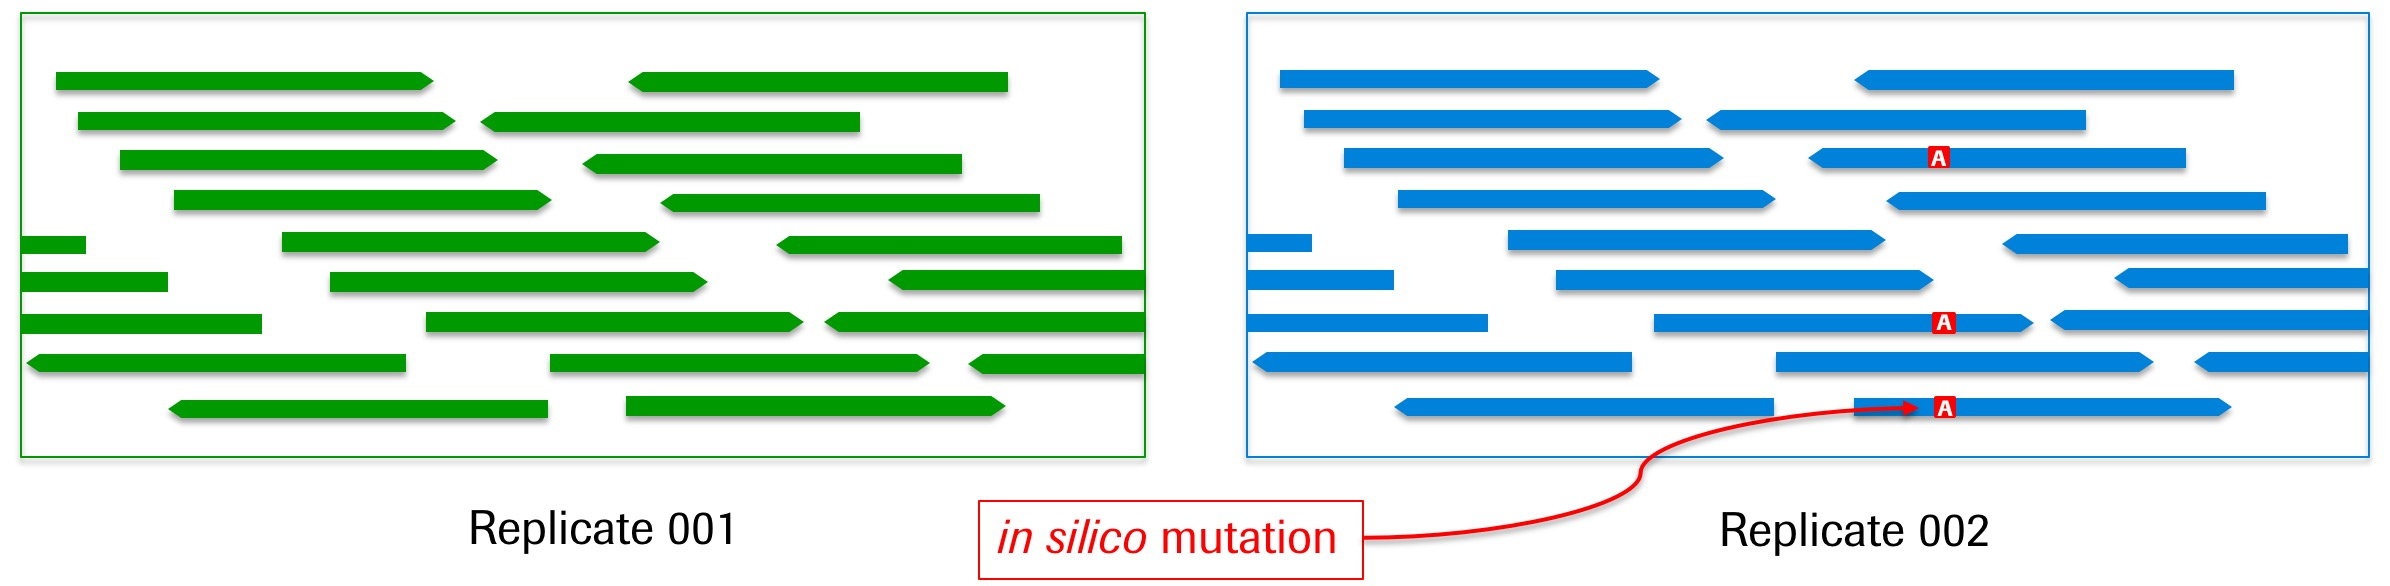
\includegraphics[width=6.5in]{../utilities/dockered_pipelines/bamSimulator/replicate_sim.jpg}
 % replicate_sim.jpg: 2390x586 px, 144dpi, 42.16x10.34 cm, bb=0 0 1195 293
\end{center}





\subsubsection{This example mimicks DREAM Challenge}

\href{https://www.synapse.org/#!Synapse:syn312572/wiki/70726}{DREAM Somatic Mutation Calling Challenge} was an international competition to find algorithms that gave the most accurate performances. 

In that case, a high-coverage BAM file is randomly split into two. One of which is designated normal, and the other one is designated tumor where mutations will be spiked in. Like the previous example, any mutations found between the designated tumor and designated normal are false positive, since not only are they from the same sample, but also from the same sequencing run. This example will not capture false positives as a result of run-to-run biases if they exist in your sequencing data. It will, however, still capture artefacts related to sequencing errors, sampling errors, mapping errors, etc.


\begin{lstlisting}
$PATH/TO/somaticseq/utilities/dockered_pipelines/bamSimulator/BamSimulator_multiThreads.sh \
--genome-reference /ABSOLUTE/PATH/TO/GRCh38.fa --tumor-bam-in /ABSOLUTE/PATH/TO/highCoverageGenome.bam --tumor-bam-out syntheticTumor.bam --normal-bam-out syntheticNormal.bam --split-proportion  0.5 --num-snvs 10000 --num-indels 8000 --num-svs 1500 --min-vaf 0.0 --max-vaf 1.0 --left-beta 2 --right-beta 5 --min-variant-reads 2 --output-dir /ABSOLUTE/PATH/TO/trainingSet --threads 24 --action qsub --split-bam --indel-realign --merge-output-bams
\end{lstlisting}

The --split-bem will randomly split the high coverage BAM file into two BAM files, one of which is designated normal and the other one designated tumor for mutation spike in. The --indel-realign is an option that will perform GATK Joint Indel Realignment on the two BAM files. You may or may not invoke it depending on your real data sets. The --merge-output-bams creates another script that will merge the BAM and VCF files region-by-region. It will need to be run manually after all the spike in is done.

A schematic of the DREAM Challenge simulation procedure

\begin{center}
 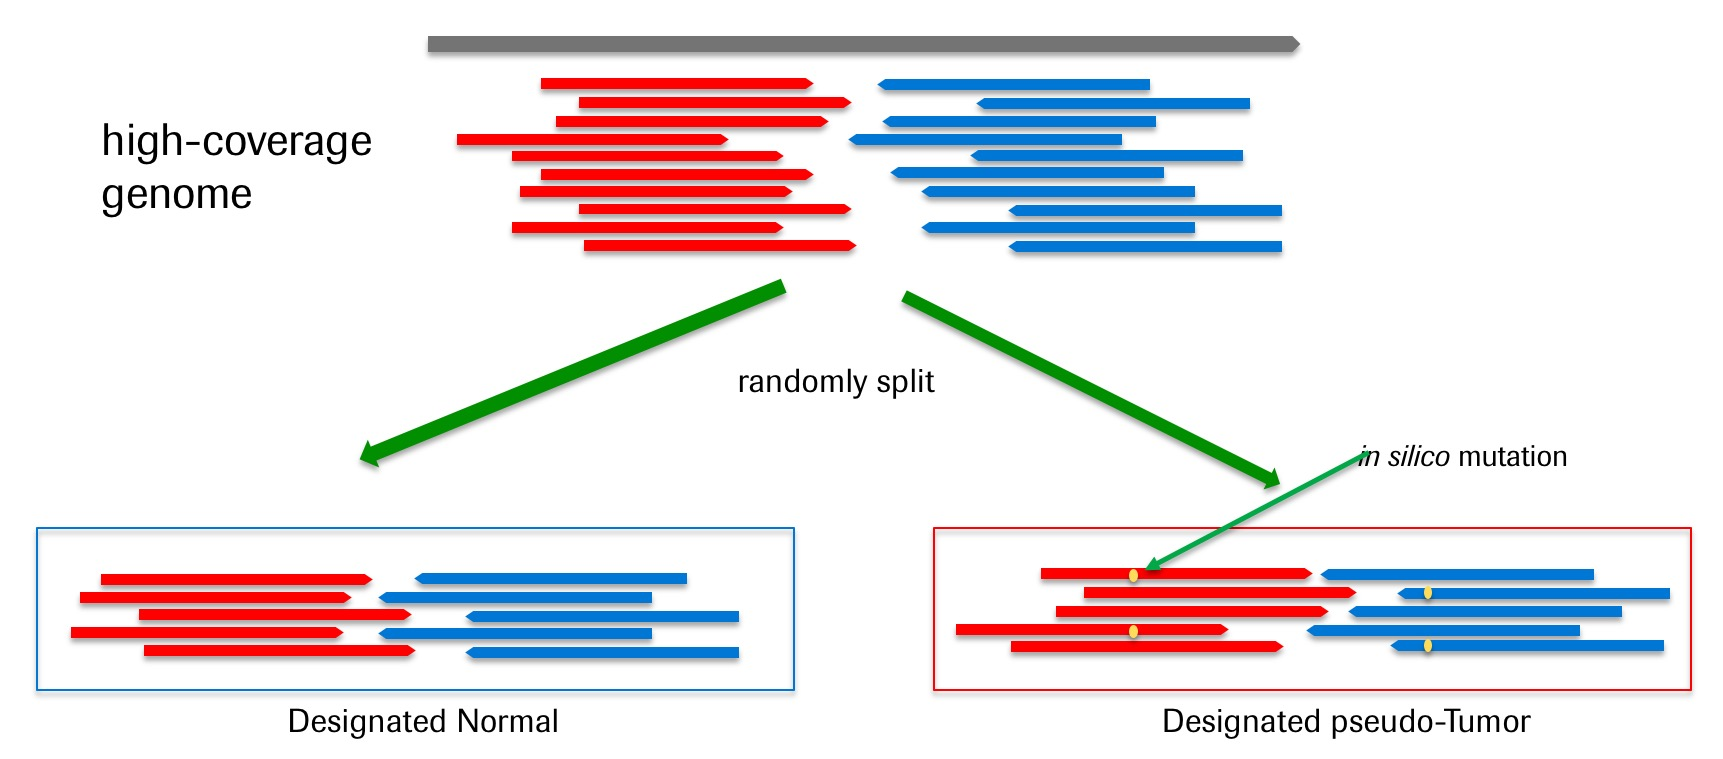
\includegraphics[width=6.5in]{../utilities/dockered_pipelines/bamSimulator/dream_sim.jpg}
 % dream_sim.jpg: 2198x660 px, 144dpi, 38.77x11.64 cm, bb=0 0 1099 330
\end{center}



\subsubsection{Merge and then split the input tumor and normal BAM files}

\begin{lstlisting}
$PATH/TO/somaticseq/utilities/dockered_pipelines/bamSimulator/BamSimulator_multiThreads.sh \
--genome-reference /ABSOLUTE/PATH/TO/GRCh38.fa --tumor-bam-in /ABSOLUTE/PATH/TO/Tumor_Sample.bam --normal-bam-in /ABSOLUTE/PATH/TO/Normal_Sample.bam --tumor-bam-out syntheticTumor.bam --normal-bam-out    syntheticNormal.bam --split-proportion  0.5 --num-snvs 30000 --num-indels 10000 --num-svs 1500 --min-vaf 0.0 --max-vaf 1.0 --left-beta 2 --right-beta 5 --min-variant-reads 2 --output-dir /ABSOLUTE/PATH/TO/trainingSet --threads 24 --action qsub --merge-bam --split-bam --indel-realign --merge-output-bams
\end{lstlisting}

The --merge-bam will merge the normal and tumor BAM files into a single BAM file. Then, --split-bem will randomly split the merged BAM file into two BAM files. One of which is designated normal, and one of which is designated tumor. Synthetic mutations will then be spiked into the designated tumor to create "real" mutations. This is the approach described in our \href{http://dx.doi.org/10.1158/1538-7445.AM2017-386}{2017 AACR Abstract}.


A schematic of the simulation procedure

\begin{center}
 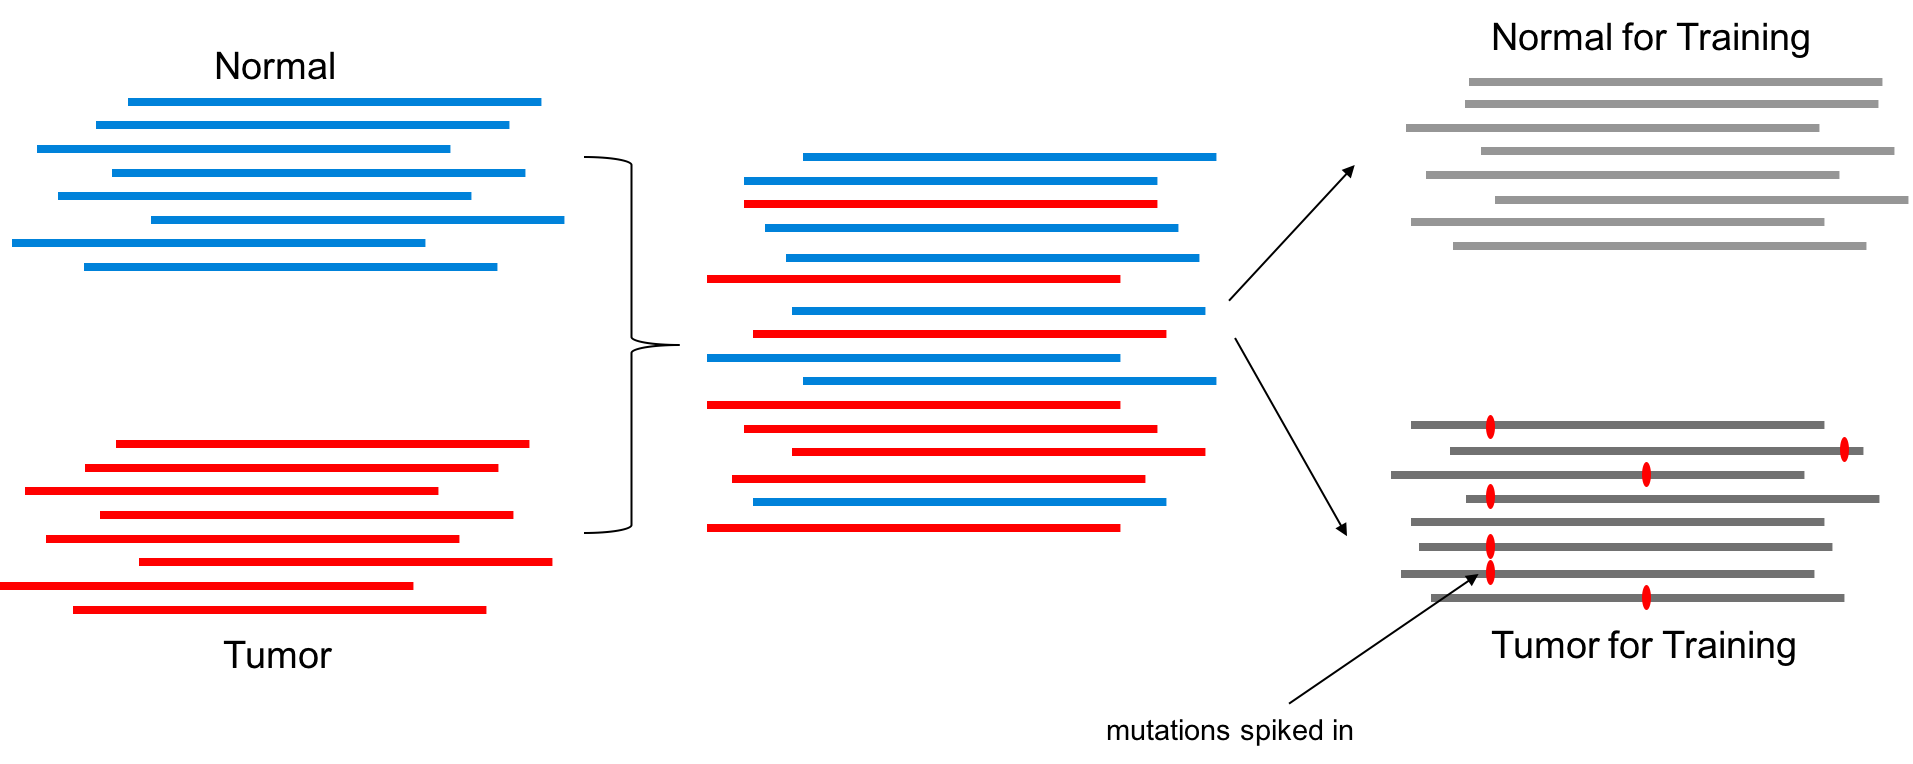
\includegraphics[width=6.5in]{../utilities/dockered_pipelines/bamSimulator/onkoinsight_sim.png}
 % onkoinsight_sim.png: 1913x764 px, 150dpi, 32.39x12.94 cm, bb=0 0 918 367
\end{center}


\subsection{Parameters and Options}

\begin{lstlisting}
--genome-reference  /ABSOLUTE/PATH/TO/human_reference.fa (Required)
--selector          /ABSOLUTE/PATH/TO/capture_region.bed (BED file to limit where mutation spike in will be attempted)
--tumor-bam-in      Input BAM file (Required)
--normal-bam-in     Input BAM file (Optional, but required if you want to merge it with the tumor input)
--tumor-bam-out     Output BAM file for the designated tumor after BAMSurgeon mutation spike in
--normal-bam-out    Output BAM file for the designated normal if --split-bam is chosen
--split-proportion  The faction of total reads desginated to the normal. (Defaut = 0.5)
--num-snvs          Number of SNVs to spike into the designated tumor
--num-indels        Number of INDELs to spike into the designated tumor
--num-svs           Number of SVs to spike into the designated tumor (Default = 0)
--min-depth         Minimum depth where spike in can take place
--max-depth         Maximum depth where spike in can take place
--min-vaf           Minimum VAF to simulate
--max-vaf           Maximum VAF to simulate
--left-beta         Left beta of beta distribution for VAF
--right-beta        Right beta of beta distribution for VAF
--min-variant-reads Minimum number of variant-supporting reads for a successful spike in
--output-dir        Output directory
--merge-bam         Flag to merge the tumor and normal bam file input
--split-bam         Flag to split BAM file for tumor and normal
--clean-bam         Flag to go through the BAM file and remove reads where more than 2 identical read names are present, or reads where its read length and CIGAR string do not match. This was necessary for some BAM files downloaded from TCGA. However, a proper pair-end BAM file should not have the same read name appearing more than twice. Use this only when necessary as it first sorts BAM file by qname, goes through the cleaning procedure, then re-sort by coordinates.
--indel-realign     Conduct GATK Joint Indel Realignment on the two output BAM files. Instead of syntheticNormal.bam and syntheticTumor.bam, the final BAM files will be syntheticNormal.JointRealigned.bam and syntheticTumor.JointRealigned.bam.
--seed              Random seed. Pick any integer for reproducibility purposes.
--threads           Split the BAM files evenly in N regions, then process each (pair) of sub-BAM files in parallel. 
--action            The command preceding the run script created into /ABSOLUTE/PATH/TO/BamSurgeoned_SAMPLES/logs. "qsub" is to submit the script in SGE system. Default = echo
\end{lstlisting}


\subsubsection{--merge-bam / --split-bam / --indel-realign}


If you have sequenced replicate normal, that's the best data set for training. You can use one of the normal as normal, and designate the other normal (of the same sample) as tumor. Use --indel-realign to invoke GATK IndelRealign.

When you have a normal that's roughly 2X the coverage as your data of choice, you can split that into two halves. One designated as normal, and the other one designated as tumor. That DREAM Challenge's approach. Use --split-bam --indel-realign options.

Another approach is to merge the tumor and normal data, and then randomly split them as described above. When you merge the tumor and normal, the real tumor mutations are relegated as germline or noise, so they are considered false positives, because they are supposed to be evenly split into the designated normal. To take this approach, use --merge-bam --split-bam --indel-realign options.

Don't use --indel-realign if you do not use indel realignment in your alignment pipeline.

In some BAM files, there are reads where read lengths and CIGAR strings don't match. Spike in will fail in these cases, and you'll need to invoke --clean-bam to get rid of these problematic reads.

You can control and visualize the shape of target VAF distribution with python command:

\begin{lstlisting}
    import scipy.stats as stats
    import numpy as np
    import matplotlib.pyplot as plt

    leftBeta, rigthBeta = 2,5
    minAF, maxAF = 0,1
    x = np.linspace(0,1,101)
    y = stats.beta.pdf(x, leftBeta, rigthBeta, loc = minAF, scale = minAF + maxAF)
    _ = plt.plot(x, y)
\end{lstlisting}


\subsection{To create SomaticSeq classifiers}

After the mutation simulation jobs are completed, you may create classifiers with the training data with the following command:

See our \href{https://github.com/bioinform/somaticseq/blob/master/utilities/dockered_pipelines}{somatic mutation pipeline} for more details.

\begin{lstlisting}
$PATH/TO/somaticseq/utilities/dockered_pipelines/submit_callers_multiThreads.sh \
--output-dir      /ABSOLUTE/PATH/TO/trainingSet/somaticMutationPipeline \
--normal-bam      /ABSOLUTE/PATH/TO/trainingSet/syntheticNormal.bam \
--tumor-bam       /ABSOLUTE/PATH/TO/trainingSet/syntheticTumor.bam \
--human-reference /ABSOLUTE/PATH/TO/GRCh38.fa \
--dbsnp           /ABSOLUTE/PATH/TO/dbSNP.GRCh38.vcf \
--thread          24 \
--truth-snv       /ABSOLUTE/PATH/TO/trainingSet/synthetic_snvs.vcf \
--truth-indel     /ABSOLUTE/PATH/TO/trainingSet/synthetic_indels.leftAlign.vcf \
--action          echo \
--mutect2 --somaticsniper --vardict --muse --lofreq --strelka --somaticseq
\end{lstlisting}





\section{Release Notes}

Make sure training and prediction use the same SomaticSeq version, or at least make sure the different minor version changes do not change the results significantly. 


\subsection{Version 1.0}
Version used to generate data in the manuscript and \href{https://www.synapse.org/#!Synapse:syn312572/wiki/72943}{Stage 5 of the ICGC-TCGA DREAM Somatic Mutation Challenge}, where SomaticSeq's results were \#1 for INDEL and \#2 for SNV. 

In the original manuscript, VarDict's var2vcf\_somatic.pl script was used to generate VarDict VCFs, and subsequently ``-filter somatic'' was used for SSeq\_merged.vcf2tsv.py. Since then (including DREAM Challenge Stage 5), VarDict recommends var2vcf\_paired.pl over var2vcf\_somatic.pl, and subsequently ``-filter paired'' was used for SSeq\_merged.vcf2tsv.py. The difference in SomaticSeq results, however, is pretty much negligible. 

\subsection{Version 1.1}
Automated the SomaticSeq.Wrapper.sh script for both training and prediction mode. No change to any algorithm. 

\subsection{Version 1.2}
Have implemented the following improvement, mostly for indels:

\begin{itemize}
 
  \item 
  SSeq\_merged.vcf2tsv.py can now accept pileup files to extract read depth and DP4 (reference forward, reference reverse, alternate forward, and alternate reverse) information (mainly for indels). Previously, that information can only be extracted from SAMtools VCF. Since the SAMtools or HaplotypeCaller generated VCFs hardly contain any indel information, this option improves the indel model. The SomaticSeq.Wrapper.sh script is modified accordingly.
 
  \item
  Extract mapping quality (MQ) from VarDict output if this information cannot be found in SAMtools VCF (also mostly benefits the indel model). 
 
  \item
  Indel length now positive for insertions and negative for deletions, instead of using the absolute value previously. 
 
 
\end{itemize}




\subsection{Version 2.0}

\begin{itemize}
  \item
  Removed dependencies for SAMtools and HaplotypeCaller during feature extraction. SSeq\_merged.vcf2tsv.py extracts those information (plus more) directly from BAM files.

  \item
  Allow not only VCF file, but also BED file or a list of chromosome coordinate as input format for SSeq\_merged.vcf2tsv.py, i.e., use -mybed or -mypos instead of -myvcf. 

  \item
  Instead of a separate step to annotate ground truth, that can be done directly by SSeq\_merged.vcf2tsv.py by supplying the ground truth VCF via -truth.

  \item
  SSeq\_merged.vcf2tsv.py can annotate dbSNP and COSMIC information directly if BED file or a list of chromosome coordinates are used as input in lieu of an annotated VCF file. 

  \item
  Consolidated feature sets, e.g., removed some redunda
  Fixed a bug: if JointSNVMix2 is not included, the values should be ``NaN'' instead of 0's. This is to keep consistency with how we handle all other callersnt feature sets coming from different resources.
\end{itemize}


\subsection{Version 2.0.2}

\begin{itemize}

  \item
  Incorporated LoFreq.
  
  \item
  Used getopt to replace getopts in the SomaticSeq.Wrapper.sh script to allow long options. 
  
\end{itemize}



\subsection{Version 2.1.2}

\begin{itemize}

  \item
  Properly handle cases when multiple ALT's are calls in the same position. The VCF files can either contain multiple calls in the ALT column (i.e., A,G), or have multiple lines corresponding to the same position (one line for each variant call). Some functions were significantly re-written to allow this.

  \item
  Incorporated Scalpel.
  
  \item
  Deprecated HaplotypeCaller and SAMTools dependencies completely as far as feature generation is concerned.
  
  \item
  The Wrapper script removed SnpSift/SnpEff dependencies. Those information can be directly obtained during the SSeq\_merged.vcf2tsv.py step. Also removed some additional legacy steps that has become useless since v2 (i.e., score\_Somatic.Variants.py). Added a step to check the correctness of the input. The v2.1 and 2.1.1 had some typos in the wrapper script, so only describing v2.1.2 here.

\end{itemize}



\subsection{Version 2.2}

\begin{itemize}

  \item
  Added MuTect2 support.

\end{itemize}



\subsection{Version 2.2.1}

\begin{itemize}

  \item
  InDel\_3bp now stands for indel counts within 3 bps of the variant site, instead of exactly 3 bps from the variant site as it was previously (likewise for InDel\_2bp). 
 
  \item
  Collapse MQ0 (mapping quality of 0) reads supporting reference/variant reads into a single metric of MQ0 reads (i.e., tBAM\_MQ0 and nBAM\_MQ0). From experience, the number of MQ0 reads is at least equally predictive of false positive calls, rather than distinguishing if those MQ0 reads support reference or variant. 
  
  \item
  Obtain SOR (Somatic Odds Ratio) from BAM files instead of VarDict's VCF file.
  
  \item
  Fixed a typo in the SomaticSeq.Wrapper.sh script that did not handle inclusion region correctly.
  
\end{itemize}



\subsection{Version 2.2.2}

\begin{itemize}

  \item
  Got around an occasional unexplained issue in then ada package were the SOR is sometimes categorized as type, by forcing it to be numeric. 
  
  \item
  Defaults PASS score from 0.7 to 0.5, and make them tunable in the SomaticSeq.Wrapper.sh script (\texttt{--}pass-threshold and \texttt{--}lowqual-threshold). 
  
\end{itemize}



\subsection{Version 2.2.3}

\begin{itemize}

  \item
  Incorporated Strelka2 since it's now GPLv3.
  
  \item
  Added another R script (ada\_model\_builder\_ntChange.R) that uses nucleotide substitution pattern as a feature. Limited experiences have shown us that it improves the accuracy, but it's not heavily tested yet. 

  \item
  If a COSMIC site is labeled SNP in the COSMIC VCF file, if\_cosmic and CNT will be labeled as 0. The COSMIC ID will still appear in the ID column. This will not change any results because both of those features are turned off in the training R script.
  
  \item
  Fixed a bug: if JointSNVMix2 is not included, the values should be ``NaN'' instead of 0's. This is to keep consistency with how we handle all other callers.
  
\end{itemize}



\subsection{Version 2.2.4}

\begin{itemize}

  \item
  Resolved a bug in v2.2.3 where the VCF files of Strelka INDEL and Scalpel clash on GATK CombineVariants, by outputting a temporary VCF file for Strelka INDEL without the sample columns.
  
  \item
  Caller classification: consider if\_Scalpel = 1 only if there is a SOMATIC flag in its INFO. 

\end{itemize}


\subsection{Version 2.2.5}

\begin{itemize}
  
  \item
  Added a dockerfile. Docker repo at https://hub.docker.com/r/lethalfang/somaticseq/. 
  
  \item
  Ability to use vcfsort.pl instead of GATK CombineVariants to merge VCF files.

\end{itemize}


\subsection{Version 2.3.0}

\begin{itemize}
  
  \item
  Moved some scripts to the utilities directory to clean up the clutter.
  
  \item
  Added the split\_Bed\_into\_equal\_regions.py to utilities, which will split a input BED file into multiple BED files of equal size. This is to be used to parallelize large WGS jobs.
  
  \item
  Made compatible with MuTect2 from GATK4.
  
  \item
  Removed long options for the SomaticSeq.Wrapper.sh script because it's more readable this way.
  
  \item
  Added a script to add ``GT'' field to Strelka's VCF output before merging it with other VCF files. That was what caused GATK CombineVariants errors mentioned in v2.2.4's release notes. 
  
  \item
  Added a bunch of scripts at utilities/dockered\_pipelines that can be used to submit (requiring Sun Grid Engine or equivalent) dockerized pipeline to a computing cluster. 

\end{itemize}


\subsection{Version 2.3.1}

\begin{itemize}

  \item
  Improve the automated run script generator at utilities/dockered\_pipelines.
  
  \item
  No change to SomaticSeq algorithm

\end{itemize}



\subsection{Version 2.3.2}

\begin{itemize}

  \item
  Added run script generators for dockerized BAMSurgeon pipelines at utilities/dockered\_pipelines/bamSurgeon
  
  \item
  Added an error message to r\_scripts/ada\_model\_builder\_ntChange.R when TrueVariants\_or\_False don't have both 0's and 1's. Other than this warning message change, no other change to SomaticSeq algorithm.  

\end{itemize}


\subsection{Version 2.4.0}

\begin{itemize}

  \item
  Restructured the utilities scripts.
  
  \item
  Added the utilities/filter\_SomaticSeq\_VCF.py script that ``demotes'' PASS calls to LowQual based on a set of tunable hard filters.
  
  \item
  BamSurgeon scripts invokes modified BamSurgeon script that splits a BAM file without the need to sort by read name. This works if the BAM files have proper read names, i.e., 2 and only 2 identical read names for each paired-end reads.
  
  \item
  No change to SomaticSeq algorithm

\end{itemize}



\subsection{Version 2.4.1}

\begin{itemize}

  \item
  Updated some docker job scripts.
  
  \item
  Added a script that converts some items in the VCF's INFO field into the sample field, to precipitate the need to merge multiple VCF files into a single multi-sample VCF, i.e., utilities/reformat\_VCF2SEQC2.py.
  
  \item
  No change to SomaticSeq algorithm

\end{itemize}




\subsection{Version 2.5.0}

\begin{itemize}

  \item
  In modify\_VJSD.py, get rid of VarDict's END tag (in single sample mode) because it causes problem with GATK CombineVariants. 
  
  \item
  Added limited single-sample support, i.e., ssSomaticSeq.Wrapper.sh is the wrapper script. singleSample\_callers\_singleThread.sh is the wrapper script to submit single-sample mutation caller scripts.
  
  \item
  Added run scripts for read alignments and post-alignment processing, i.e,. FASTQ $\rightarrow$ BAM, at utilities/dockered\_pipelines/alignments.
  
  \item
  Fixed a bug where the last two CD4 numbers were both alternate concordant reads in the output VCF file, when the last number should've been alternate discordant reads.
  
  \item
  Changed the output file names from Trained.s(SNV$\vert$INDEL).vcf and Untrained.s(SNV$\vert$INDEL).vcf to SSeq.Classified.s(SNV$\vert$INDE).vcf and Consensus.s(SNV$\vert$INDEL).vcf. No change to the actual tumor-normal SomaticSeq algorithm.
  
  \item
  Added utilities/modify\_VarDict.py to VarDict's ``complex'' variant calls (e.g., GCA>TAC) into SNVs when possible. 
  
  \item
  Modified r\_scripts/ada\_model\_builder\_ntChange.R to allow you to ignore certain features, e.g., r\_scripts/ada\_model\_builder\_ntChange.R Training\_Data.tsv nBAM\_REF\_BQ tBAM\_REF\_BQ SiteHomopolymer\_Length ...
  
  Everything after the input file are features to be ignored during training.
  
  Also added r\_scripts/ada\_cross\_validation.R.

\end{itemize}



\subsection{Version 2.5.1}

\begin{itemize}
  \item
  Additional passable parameters options to pass extra parameters to somatic mutation callers. Fixed a bug where the ``two-pass'' parameter is not passed onto Scalpel in multiThreads scripts. 
  
  \item
  Ignore Strelka\_QSS and Strelka\_TQSS for indel training in the SomaticSeq.Wrapper.sh script.
  
\end{itemize}



\subsection{Version 2.5.2}

\begin{itemize}
  \item
  Ported some pipeline scripts to singularities at utilities/singularities.
  
\end{itemize}


\subsection{Version 2.6.0}

\begin{itemize}
  \item
  VarScan2\_Score is no longer extracted from VarScan's output. Rather, it's now calculated directly using Fisher's Exact Test, which reproduces VarScan's output, but will have a real value when VarScan2 does not output a particular variant. 
  
  \item
  Incorporate TNscope's output VCF into SomaticSeq, but did not incorporate TNscope caller into the dockerized workflow because we don't have distribution license. 
  
\end{itemize}



\subsection{Version 2.6.1}

\begin{itemize}
  \item
  Optimized memory for singularity scripts.
  
  \item
  Updated utilities/bamQC.py and added utilities/trimSoftClippedReads.py (removed soft-clipped bases on soft-clipped reads)
  
  \item
  Added some docker scripts at utilities/dockered\_pipelines/QC

\end{itemize}


\subsection{Version 2.7.0}

\begin{itemize}
  \item
  Added another feature: consistent/inconsistent calls for paired reads if the position is covered by both forward and reverse reads. However, they're excluded as training features in SomaticSeq.Wrapper.sh script for the time being. 
  
  \item
  Change non-GCTA characters to N in VarDict.vcf file to make it conform to VCF file specifications. 

\end{itemize}


\subsection{Version 2.7.1}

\begin{itemize}

  \item
  Without --gatk \$PATH/TO/GenomeAnalysisTK.jar in the SomaticSeq.Wrapper.sh script, it will use utilities/getUniqueVcfPositions.py and utilities/vcfsorter.pl to (in lieu of GATK3 CombineVariants) to combine all the VCF files. 

  \item
  Fixed bugs in the docker/singularities scripts where extra arguments for the callers are not correctly passed onto the callers. 

\end{itemize}




\subsection{Version 2.7.2}

\begin{itemize}

  \item
  Make compatible with .cram format
  
  \item
  Fixed a bug where Strelka-only calls are not considered by SomaticSeq. 
  
\end{itemize}



\subsection{Version 2.8.0}

\begin{itemize}

  \item
  The program is now designed to crash if the VCF file(s) are not sorted according to the .fasta reference file. 
  
\end{itemize}



\section{Contact Us}
For suggestions, bug reports, or technical support, please post in \href{https://github.com/bioinform/somaticseq/issues}{https://github.com/bioinform/somaticseq/issues}. The developers are alerted when issues are created there. Alternatively, you may also email \href{mailto:li_tai.fang@roche.com}{li\_tai.fang@roche.com}. 

\end{sloppypar}
\end{document}
